\chapter{Le tableau d'avancement}\label{ch:g10:reaction-progress-table}

% ledger: use:NaN3-airbag
Lors d'un accident de voiture, un coussin jaillit du volant et se remplit
de gaz en une fraction de seconde, avant que la tête du conducteur ne
parte vers l'avant. Le gaz est produit par une \omterm{def:g7:chemical-reactions:reaction}{réaction chimique}~: une
petite charge de solide, de l'azoture de sodium dans la conception
classique, se décompose en sodium et en diazote. L'ingénieur doit mettre
assez de solide pour remplir le coussin, mais pas au point de le faire
éclater, et aucun \omterm{def:g7:chemical-reactions:reactant}{réactif} ne doit rester pour nuire aux passagers.
Quelle masse de solide donne quel volume de gaz~? Une \omterm{def:g8:balanced-equations:equation}{équation ajustée}
donne les proportions~; ce chapitre en fait un outil de comptabilité qui
suit chaque \omterm{def:g7:chemical-reactions:reactant}{réactif} et chaque produit du début à la fin d'une réaction.

\begin{recall}
Une \omterm{def:g8:balanced-equations:equation}{équation ajustée} conserve, de part et d'autre, le nombre d'\omterm{def:g7:atoms-and-molecules:atom}{atomes} de
chaque élément et la charge~; ses coefficients donnent les proportions
dans lesquelles les espèces réagissent (\cref{ch:g8:balanced-equations}).
La \omterm{def:g10:the-mole:amount}{quantité de matière} d'une espèce vaut $n = m/M$ pour une masse,
$n = V/V_m$ pour un gaz (avec
$V_m = \qty{24.1}{L/mol}$ à \qty{20}{\celsius} et sous la pression
atmosphérique normale) (\cref{ch:g10:the-mole}), et $n = c \times V$
pour un \omterm{def:g6:solutions-and-solubility:solute}{soluté} (\cref{ch:g10:concentration-and-dilution}).
\end{recall}

\begin{omfigure}
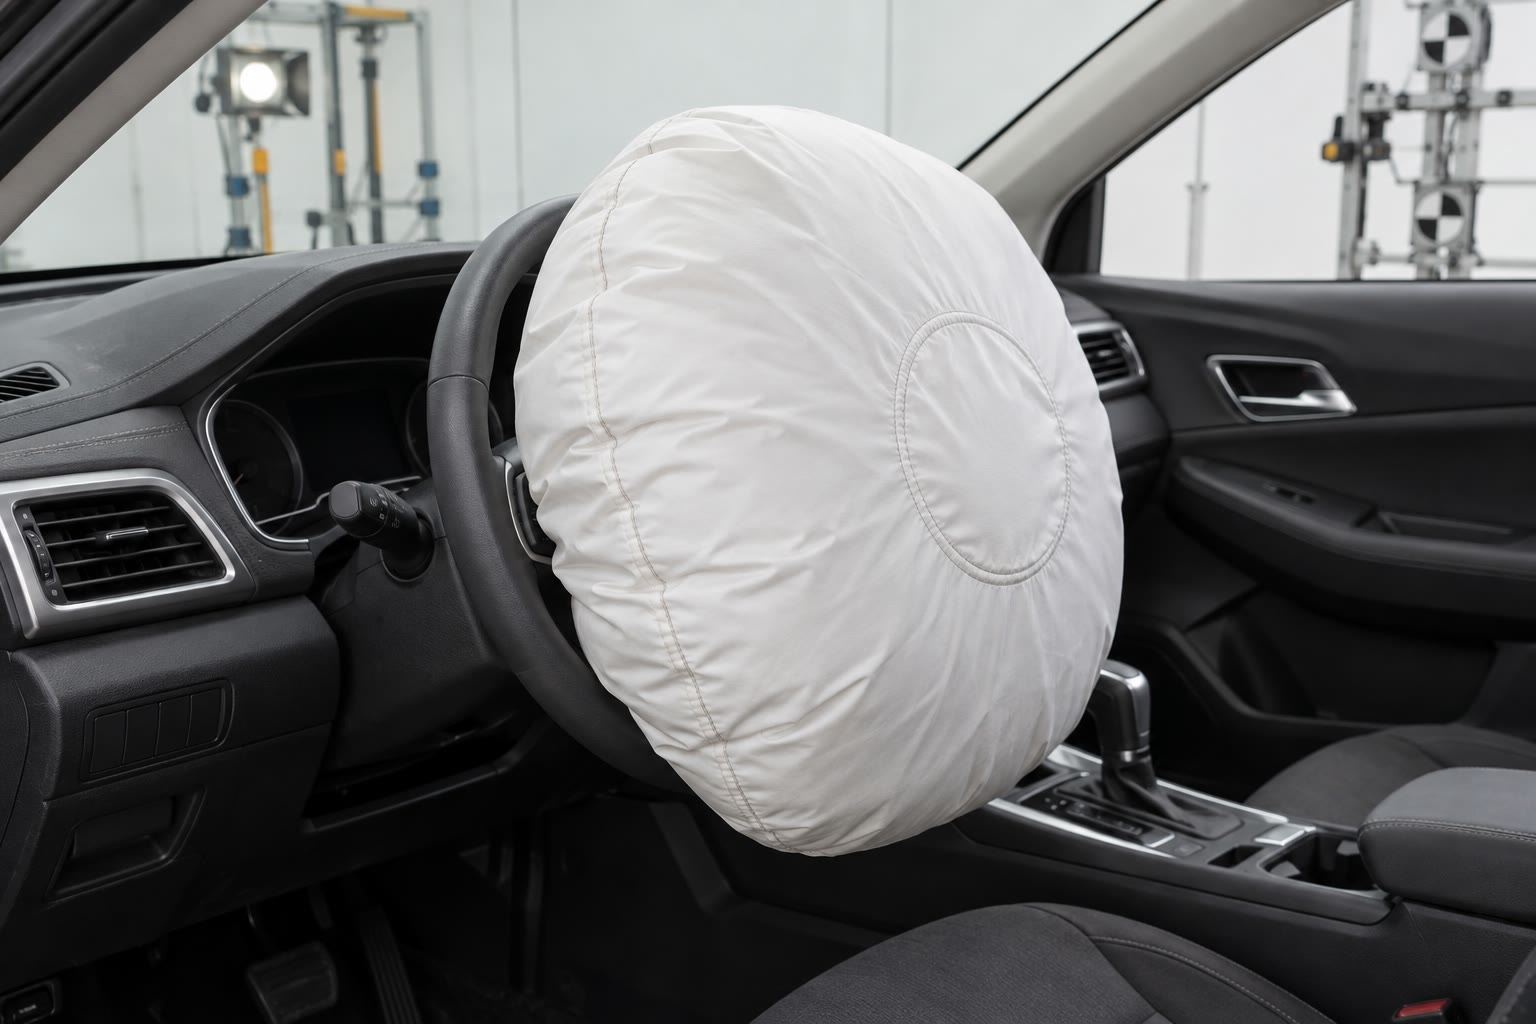
\includegraphics[width=0.5\linewidth]{images/book1/ai/g10-airbag.jpg}

{\small Un airbag se gonfle en une fraction de seconde, grâce au diazote
produit par une réaction.}
\end{omfigure}

\section{Décrire un système chimique}

\begin{definition}[Système chimique, état initial et état final]\label{def:g10:reaction-progress-table:system}
Un \emph{système chimique}\index{systeme chimique@système chimique} est l'ensemble des
\omterm{def:g6:pure-substances-and-mixtures:species}{espèces chimiques} présentes en un lieu donné (un ballon, un coussin, une
pile), chacune avec sa \omterm{def:g10:the-mole:amount}{quantité de matière} et son état physique. Le
système avant le début de la réaction est l'\emph{état
initial}\index{etat initial@état initial}~; le système une fois la réaction arrêtée
est l'\emph{état final}\index{etat final@état final}.
\end{definition}


\begin{example}[Du méthane qui brûle dans un récipient fermé]\label{ex:g10:reaction-progress-table:methane}
Un récipient fermé contient \qty{2.0}{mol} de méthane et \qty{3.0}{mol}
de dioxygène~; une étincelle déclenche la \omterm{def:g4:what-a-fire-needs:burning}{combustion}
\ce{CH4 + 2O2 -> CO2 + 2H2O}. Dans l'\omterm{def:g10:reaction-progress-table:system}{état initial}, le système contient
\qty{2.0}{mol} de \ce{CH4(g)}, \qty{3.0}{mol} de \ce{O2(g)} et aucun
produit. Que contient l'\omterm{def:g10:reaction-progress-table:system}{état final}~? La suite du chapitre répond à cette
question.
\end{example}

\section{L'avancement et le tableau d'avancement}

\begin{definition}[Avancement, tableau d'avancement]\label{def:g10:reaction-progress-table:extent}
L'\emph{avancement}\index{avancement} $x$, en \omterm{def:g10:the-mole:amount}{moles}, compte combien de
fois la réaction, telle qu'elle est écrite dans l'\omterm{def:g8:balanced-equations:equation}{équation ajustée}, s'est
produite~: quand l'avancement vaut $x$, une espèce de coefficient $\nu$
a été consommée (\omterm{def:g7:chemical-reactions:reactant}{réactif}) ou formée (produit) en quantité $\nu x$. Le
\emph{tableau d'avancement}\index{tableau d'avancement} donne, sous
l'équation, la \omterm{def:g10:the-mole:amount}{quantité de matière} de chaque espèce dans l'\omterm{def:g10:reaction-progress-table:system}{état initial},
pour un avancement $x$, et dans l'\omterm{def:g10:reaction-progress-table:system}{état final}.
\end{definition}

\begin{method}[Remplir un tableau d'avancement]\label{met:g10:reaction-progress-table:fill}
\begin{enumerate}
  \item Écrire l'\omterm{def:g8:balanced-equations:equation}{équation ajustée} sur la première ligne.
  \item \omterm{def:g10:reaction-progress-table:system}{État initial} ($x = 0$)~: écrire sous l'équation la quantité
        initiale de chaque espèce.
  \item État intermédiaire (\omterm{def:g10:reaction-progress-table:extent}{avancement} $x$)~: chaque \omterm{def:g7:chemical-reactions:reactant}{réactif} de
        coefficient $\nu$ devient $n_0 - \nu x$, chaque produit
        $n_0 + \nu x$.
  \item \omterm{def:g10:reaction-progress-table:system}{État final}~: trouver $x_{\max}$ (section suivante) et le reporter
        dans les expressions de la ligne intermédiaire.
\end{enumerate}
\end{method}

\begin{omfigure}
\renewcommand{\arraystretch}{1.25}
\begin{tabular}{l|c|cccc}
\hline
équation & & \ce{CH4} & $+$ \ce{2O2} & $\longrightarrow$ \ce{CO2} & $+$ \ce{2H2O} \\
\hline
état & \omterm{def:g10:reaction-progress-table:extent}{avancement} (\si{mol}) & \multicolumn{4}{c}{\omterm{def:g10:the-mole:amount}{quantités de matière} (\si{mol})} \\
\hline
initial & $0$ & $2.0$ & $3.0$ & $0$ & $0$ \\
intermédiaire & $x$ & $2.0 - x$ & $3.0 - 2x$ & $x$ & $2x$ \\
final & $x_{\max} = 1.5$ & $0.5$ & $0$ & $1.5$ & $3.0$ \\
\hline
\end{tabular}\par\medskip

{\small Le \omterm{def:g10:reaction-progress-table:extent}{tableau d'avancement} de la \omterm{def:g4:what-a-fire-needs:burning}{combustion} du méthane de
l'exemple. Chaque colonne suit une espèce~; les coefficients 2 de
\ce{O2} et de \ce{H2O} deviennent les $2x$.}
\end{omfigure}

\section{Le réactif limitant et l'état final}

\begin{definition}[Réactif limitant, avancement maximal, réaction totale]\label{def:g10:reaction-progress-table:limiting}
Une réaction est une \emph{réaction totale}\index{reaction totale@réaction totale} si
elle ne s'arrête que lorsque l'un de ses \omterm{def:g7:chemical-reactions:reactant}{réactifs} est entièrement
consommé. Ce \omterm{def:g7:chemical-reactions:reactant}{réactif} est le \emph{réactif limitant}\index{reactif limitant@réactif limitant}~;
les autres \omterm{def:g7:chemical-reactions:reactant}{réactifs} sont en excès. L'\omterm{def:g10:reaction-progress-table:extent}{avancement} pour lequel le \omterm{def:g7:chemical-reactions:reactant}{réactif}
limitant est épuisé est l'\emph{avancement maximal}\index{avancement maximal}
$x_{\max}$~; l'\omterm{def:g10:reaction-progress-table:system}{état final} d'une réaction totale est l'état
d'\omterm{def:g10:reaction-progress-table:extent}{avancement} $x = x_{\max}$.
\end{definition}

\begin{method}[Trouver le réactif limitant]\label{met:g10:reaction-progress-table:limiting}
\begin{enumerate}
  \item Pour chaque \omterm{def:g7:chemical-reactions:reactant}{réactif}, résoudre $n_0 - \nu x = 0$~: le \omterm{def:g7:chemical-reactions:reactant}{réactif}
        serait épuisé pour $x = n_0 / \nu$.
  \item La plus petite de ces valeurs est $x_{\max}$~; le \omterm{def:g7:chemical-reactions:reactant}{réactif} qui la
        donne est le \omterm{def:g10:reaction-progress-table:limiting}{réactif limitant}.
  \item Reporter $x_{\max}$ dans la ligne intermédiaire pour obtenir
        l'\omterm{def:g10:reaction-progress-table:system}{état final}~; vérifier qu'aucune quantité n'est négative.
\end{enumerate}
\end{method}

\begin{example}[Retour au méthane]\label{ex:g10:reaction-progress-table:methane-final}
Le méthane serait épuisé pour $x = 2.0/1 = \qty{2.0}{mol}$, le
dioxygène pour $x = 3.0/2 = \qty{1.5}{mol}$. La plus petite valeur est
\qty{1.5}{mol}~: le dioxygène est le \omterm{def:g10:reaction-progress-table:limiting}{réactif limitant} et
$x_{\max} = \qty{1.5}{mol}$. L'\omterm{def:g10:reaction-progress-table:system}{état final} contient \qty{0.5}{mol} de
méthane restant, pas de dioxygène, \qty{1.5}{mol} de dioxyde de
carbone et \qty{3.0}{mol} d'eau.
\end{example}

\begin{omfigure}
\begin{tikzpicture}
\begin{axis}[width=0.78\linewidth, height=6.2cm, xmin=0, xmax=2.05,
    ymin=0, ymax=4.2, xlabel={avancement $x$ (\si{mol})},
    ylabel={quantité de matière (\si{mol})}, axis lines*=left, ymajorgrids,
    grid style={gray!20}, tick label style={font=\small},
    label style={font=\small}, xtick={0,0.5,1,1.5,2},
    legend style={font=\small, at={(1.02,0.5)}, anchor=west, draw=none},
    legend cell align=left]
  \addplot[very thick, omDef, domain=0:2] {2-x};
  \addplot[very thick, omThm, domain=0:1.5] {3-2*x};
  \addplot[very thick, omMeth, domain=0:2] {x};
  \addplot[very thick, omProp, domain=0:2] {2*x};
  \legend{\ce{CH4}, \ce{O2}, \ce{CO2}, \ce{H2O}}
  \addplot[dashed, black!60] coordinates {(1.5,0) (1.5,4.2)};
  \node[font=\small, anchor=south west] at (axis cs:1.5,3.55) {$x_{\max}$};
  \fill[black!8, opacity=0.6] (axis cs:1.5,0) rectangle (axis cs:2.05,4.2);
\end{axis}
\end{tikzpicture}

{\small Les \omterm{def:g10:the-mole:amount}{quantités de matière} en fonction de l'\omterm{def:g10:reaction-progress-table:extent}{avancement} pour
l'exemple du méthane. Le dioxygène (en rouge) atteint zéro le premier,
pour $x = \qty{1.5}{mol}$~: la réaction s'arrête là, et la partie grisée
n'est jamais atteinte.}
\end{omfigure}

\begin{remark}[Toutes les réactions ne sont pas totales]\label{rem:g10:reaction-progress-table:not-total}
Beaucoup de réactions s'arrêtent avant qu'aucun \omterm{def:g7:chemical-reactions:reactant}{réactif} soit épuisé~:
elles atteignent un état où \omterm{def:g7:chemical-reactions:reactant}{réactifs} et produits coexistent. Leur \omterm{def:g10:reaction-progress-table:system}{état
final} n'est pas $x_{\max}$, et un chapitre suivant apprend à le
trouver. Dans ce chapitre, toutes les réactions sont totales.
\end{remark}

\section{Le mélange stœchiométrique}

\begin{definition}[Mélange stœchiométrique]\label{def:g10:reaction-progress-table:stoichiometric}
Un \omterm{def:g6:pure-substances-and-mixtures:mixture}{mélange} de \omterm{def:g7:chemical-reactions:reactant}{réactifs} est un \emph{mélange
stœchiométrique}\index{melange stoechiometrique@mélange stœchiométrique} quand les quantités
initiales sont dans les proportions des coefficients de l'\omterm{def:g8:balanced-equations:equation}{équation
ajustée}.
\end{definition}

\begin{proposition}[Tous les réactifs s'épuisent ensemble]\label{prop:g10:reaction-progress-table:together}
Pour une réaction $a\,\ce{A} + b\,\ce{B} \longrightarrow$ produits, le
\omterm{def:g6:pure-substances-and-mixtures:mixture}{mélange} est stœchiométrique si et seulement si
\[
  \frac{n_0(\ce{A})}{a} = \frac{n_0(\ce{B})}{b},
\]
et alors, pour une \omterm{def:g10:reaction-progress-table:limiting}{réaction totale}, les deux \omterm{def:g7:chemical-reactions:reactant}{réactifs} sont entièrement
consommés dans l'\omterm{def:g10:reaction-progress-table:system}{état final}.
\end{proposition}

\begin{proof}
\ce{A} serait épuisé pour $x = n_0(\ce{A})/a$, \ce{B} pour
$x = n_0(\ce{B})/b$. Les deux valeurs sont égales exactement quand les
proportions sont celles de l'équation, et l'\omterm{def:g10:reaction-progress-table:extent}{avancement} $x_{\max}$ épuise
alors les deux à la fois.
\end{proof}

\begin{example}[Brûler proprement le méthane]\label{ex:g10:reaction-progress-table:stoich}
Pour \ce{CH4 + 2O2 -> CO2 + 2H2O}, \qty{2.0}{mol} de méthane demandent
\qty{4.0}{mol} de dioxygène~: $2.0/1 = 4.0/2$. Avec seulement
\qty{3.0}{mol} de dioxygène, le \omterm{def:g6:pure-substances-and-mixtures:mixture}{mélange} du premier exemple manquait de
dioxygène~; dans une vraie flamme, c'est ce manque qui produit le
monoxyde de carbone, toxique (\cref{ch:g8:combustion-and-fuels}).
\end{example}

\section{Gaz et solutions dans le tableau}


\begin{method}[Les quantités de matière de l'état initial]\label{met:g10:reaction-progress-table:amounts}
Avant de remplir un tableau, convertir chaque grandeur donnée en
\omterm{def:g10:the-mole:amount}{quantité de matière}~: $n = m/M$ pour un solide ou un liquide pesé~;
$n = V/V_m$ pour un gaz~; $n = c \times V$ pour une espèce dissoute. À
la fin, reconvertir les quantités de l'\omterm{def:g10:reaction-progress-table:system}{état final} en ce qui est
demandé~: masse, volume de gaz ou concentration.
\end{method}

\begin{example}[Le magnésium dans l'acide chlorhydrique]\label{ex:g10:reaction-progress-table:magnesium}
% ledger: aw:Mg
L'acide chlorhydrique contient des \omterm{def:g9:ions:ion}{ions} hydrogène \ce{H+}, qui attaquent
le magnésium~: \ce{Mg + 2H+ -> Mg^{2+} + H2}. On plonge un ruban de
\qty{0.12}{g} de magnésium dans \qty{50.0}{mL} d'acide de concentration
$c(\ce{H+}) = \qty{1.0}{mol/L}$. Quantités initiales~:
$n_0(\ce{Mg}) = 0.12/24.3 = \qty{4.9e-3}{mol}$ et
$n_0(\ce{H+}) = 1.0 \times 0.0500 = \qty{5.0e-2}{mol}$. Le magnésium
serait épuisé pour $x = \qty{4.9e-3}{mol}$, les \omterm{def:g9:ions:ion}{ions} hydrogène pour
$x = 0.050/2 = \qty{2.5e-2}{mol}$~: le magnésium est limitant et
$x_{\max} = \qty{4.9e-3}{mol}$. La réaction donne \qty{4.9e-3}{mol} de
dihydrogène, soit $\num{4.9e-3} \times 24.1 = \qty{0.12}{L}$ à
\qty{20}{\celsius}, et laisse $0.050 - 2 \times 0.0049 =
\qty{0.040}{mol}$ d'\omterm{def:g9:ions:ion}{ions} hydrogène en excès.
\end{example}

\begin{inthelab}[Des ballons sur des erlenmeyers]
L'enseignant verse \qty{50.0}{mL} du même acide chlorhydrique dans
chacun de six erlenmeyers, et place dans six ballons de baudruche des
masses croissantes de magnésium en poudre~: 0.15, 0.30, 0.45, 0.60, 0.75
et \qty{0.90}{g}. Chaque ballon est fixé sur le col de son erlenmeyer,
puis redressé pour que la poudre tombe dans l'acide. Les ballons se
gonflent en pétillant. Quand tout s'est arrêté, les ballons sont de plus
en plus gros du premier au quatrième erlenmeyer~; le quatrième, le
cinquième et le sixième ont la même taille, et dans les deux derniers
il reste un peu de poudre grise au fond de l'erlenmeyer.
\end{inthelab}

\begin{omfigure}
\begin{tikzpicture}[font=\small, scale=0.82]
  % H2 volume (L): 0.149 0.298 0.446 0.595 0.6025 0.6025; radius ~ V^(1/3)
  \foreach \i/\m/\v/\r/\left in {0/0.15/0.15/0.42/0, 1/0.30/0.30/0.53/0,
      2/0.45/0.45/0.61/0, 3/0.60/0.60/0.67/0, 4/0.75/0.60/0.67/1,
      5/0.90/0.60/0.67/1} {
    \begin{scope}[shift={(2.35*\i,0)}]
      \pic[transform shape] at (0,0) {erlenmeyer={0.25}{omWater}};
      \ifnum\left=1
        \fill[black!45] (-0.5,0.03) rectangle (0.5,0.12);
      \fi
      \fill[omProp!35, draw=omProp!80!black] (-0.3,2.6) -- (0.3,2.6)
        -- (0.12,2.82) -- (-0.12,2.82) -- cycle;
      \shade[ball color=omProp!40, draw=omProp!80!black]
        (0,{2.78+\r}) circle (\r);
      \node[align=center, anchor=north] at (0,-0.15)
        {\qty{\m}{g} Mg\\ \qty{\v}{L}};
    \end{scope}
  }
\end{tikzpicture}

{\small Six erlenmeyers contenant le même acide et des masses croissantes
de magnésium, avec le volume de dihydrogène (à \qty{20}{\celsius}) de
chaque ballon. Au-delà d'environ \qty{0.61}{g}, l'acide est limitant~:
les ballons cessent de grossir et il reste du magnésium (en gris).}
\end{omfigure}

\begin{remark}[Lire le palier]\label{rem:g10:reaction-progress-table:plateau}
Dans les premiers erlenmeyers, le magnésium est le \omterm{def:g10:reaction-progress-table:limiting}{réactif limitant}, et
en doubler la masse double le gaz. À partir d'une certaine masse, ce
sont les \omterm{def:g9:ions:ion}{ions} hydrogène qui s'épuisent les premiers~: ajouter du
magnésium ne change plus que la poudre restante. Le changement se
produit exactement au \omterm{def:g10:reaction-progress-table:stoichiometric}{mélange stœchiométrique},
$n_0(\ce{Mg}) = n_0(\ce{H+})/2 = \qty{0.025}{mol}$, soit
$0.025 \times 24.3 = \qty{0.61}{g}$ de magnésium.
\end{remark}

\begin{safety}{\ghs[0.82cm]{GHS02}\ghs[0.82cm]{GHS05}\ghs[0.82cm]{GHS07}}
% ledger: ghs:Mg, ghs:HCl
Le magnésium en poudre est inflammable~; l'acide chlorhydrique brûle la
peau et les yeux et ses vapeurs irritent les voies respiratoires~; le
dihydrogène \omterm{def:g4:what-a-fire-needs:burning}{brûle} dans l'\omterm{def:g4:air-a-mixture-of-gases:air}{air}. Démonstration faite par l'enseignant, avec
des lunettes, loin de toute flamme.
\end{safety}

\section{Exercices}

\begin{exercise}[$\star$]\label{exo:g10:reaction-progress-table:1}
Remplir le \omterm{def:g10:reaction-progress-table:extent}{tableau d'avancement} de \ce{2H2 + O2 -> 2H2O} pour un \omterm{def:g6:pure-substances-and-mixtures:mixture}{mélange}
initial de \qty{4.0}{mol} de dihydrogène et de \qty{3.0}{mol} de
dioxygène, en supposant la \omterm{def:g10:reaction-progress-table:limiting}{réaction totale}. Donner $x_{\max}$, le
\omterm{def:g10:reaction-progress-table:limiting}{réactif limitant} et l'\omterm{def:g10:reaction-progress-table:system}{état final}.
\end{exercise}

\begin{exercise}[$\star$]\label{exo:g10:reaction-progress-table:2}
Le carbone \omterm{def:g4:what-a-fire-needs:burning}{brûle} dans le dioxygène~: \ce{C + O2 -> CO2}. À partir de
\qty{3.0}{mol} de carbone et de \qty{2.0}{mol} de dioxygène, déterminer
$x_{\max}$, le \omterm{def:g10:reaction-progress-table:limiting}{réactif limitant} et l'\omterm{def:g10:reaction-progress-table:system}{état final}.
\end{exercise}

\begin{exercise}[$\star$]\label{exo:g10:reaction-progress-table:3}
Le fer et le soufre réagissent quand on les chauffe~: \ce{Fe + S -> FeS}.
À partir de \qty{0.50}{mol} de fer et de \qty{0.30}{mol} de soufre,
décrire l'\omterm{def:g10:reaction-progress-table:system}{état final}.
\end{exercise}

\begin{exercise}[$\star$]\label{exo:g10:reaction-progress-table:4}
On suppose la réaction \ce{N2 + 3H2 -> 2NH3} totale. À partir de
\qty{1.0}{mol} de diazote et de \qty{2.4}{mol} de dihydrogène,
déterminer $x_{\max}$ et l'\omterm{def:g10:reaction-progress-table:system}{état final}.
\end{exercise}

\begin{exercise}[$\star$]\label{exo:g10:reaction-progress-table:5}
Pour \ce{2CO + O2 -> 2CO2}, lequel de ces \omterm{def:g6:pure-substances-and-mixtures:mixture}{mélanges} est
stœchiométrique~? (a) \qty{2}{mol} de \ce{CO} et \qty{2}{mol} de
\ce{O2}~; (b) \qty{4}{mol} de \ce{CO} et \qty{2}{mol} de \ce{O2}~;
(c) \qty{1}{mol} de \ce{CO} et \qty{2}{mol} de \ce{O2}.
\end{exercise}

\begin{exercise}[$\star\star$]\label{exo:g10:reaction-progress-table:6}
Quelle masse de dioxygène faut-il pour \omterm{def:g4:what-a-fire-needs:burning}{brûler} complètement \qty{32}{g}
de méthane (\ce{CH4 + 2O2 -> CO2 + 2H2O})~? Quelle masse d'eau se
forme-t-il~?
\end{exercise}

\begin{exercise}[$\star\star$]\label{exo:g10:reaction-progress-table:7}
Un réchaud de camping \omterm{def:g4:what-a-fire-needs:burning}{brûle} \qty{1.0}{kg} de propane~:
\ce{C3H8 + 5O2 -> 3CO2 + 4H2O}. Quel volume de dioxyde de carbone, à
\qty{20}{\celsius}, libère-t-il~?
\end{exercise}

\begin{exercise}[$\star\star$]\label{exo:g10:reaction-progress-table:8}
À l'aide de la figure des \omterm{def:g10:the-mole:amount}{quantités de matière} en fonction de
l'\omterm{def:g10:reaction-progress-table:extent}{avancement} pour l'exemple du méthane, lire les quantités des quatre
espèces pour $x = \qty{1.0}{mol}$. Pourquoi la droite du dioxygène
s'arrête-t-elle à $x = \qty{1.5}{mol}$~?
\end{exercise}

\begin{exercise}[$\star\star$]\label{exo:g10:reaction-progress-table:9}
On ajoute \qty{1.30}{g} de zinc en poudre à \qty{100.0}{mL} d'une
solution bleue de sulfate de cuivre à \qty{0.10}{mol/L}. La réaction est
\ce{Zn + Cu^{2+} -> Zn^{2+} + Cu}.
Déterminer le \omterm{def:g10:reaction-progress-table:limiting}{réactif limitant}, la masse de cuivre formée et la masse de
zinc restante. La solution est-elle encore bleue à la fin~?
\end{exercise}

\begin{exercise}[$\star\star$]\label{exo:g10:reaction-progress-table:10}
On ajoute \qty{0.48}{g} de magnésium à \qty{20.0}{mL} d'acide
chlorhydrique de concentration $c(\ce{H+}) = \qty{1.0}{mol/L}$
(\ce{Mg + 2H+ -> Mg^{2+} + H2}). Quel \omterm{def:g7:chemical-reactions:reactant}{réactif} est limitant~? Quel volume
de dihydrogène recueille-t-on à \qty{20}{\celsius}~?
\end{exercise}

\begin{exercise}[$\star\star$]\label{exo:g10:reaction-progress-table:11}
Dans l'exercice~3, de quel pourcentage le \omterm{def:g7:chemical-reactions:reactant}{réactif} en excès dépasse-t-il
la quantité qui aurait donné un \omterm{def:g10:reaction-progress-table:stoichiometric}{mélange stœchiométrique}~?
\end{exercise}

\begin{exercise}[$\star\star\star$]\label{exo:g10:reaction-progress-table:12}
Un élève veut \qty{10.0}{g} d'un \omterm{def:g10:reaction-progress-table:stoichiometric}{mélange stœchiométrique} de fer et de
soufre pour \ce{Fe + S -> FeS}. Quelles masses de fer et de soufre
doit-il peser~?
\end{exercise}

\begin{exercise}[$\star\star\star$]\label{exo:g10:reaction-progress-table:13}
On chauffe fortement \qty{10.0}{g} de calcaire \ce{CaCO3}, qui se
décompose totalement~: \ce{CaCO3 -> CaO + CO2}. La chaux vive \ce{CaO}
obtenue est ensuite mise dans \qty{1.8}{g} d'eau~: \ce{CaO + H2O -> Ca(OH)2}.
\begin{enumerate}
  \item Remplir le \omterm{def:g10:reaction-progress-table:extent}{tableau d'avancement} de la première réaction~; quel
        volume de dioxyde de carbone est libéré à \qty{20}{\celsius}~?
  \item Remplir le tableau de la seconde réaction. Quel \omterm{def:g7:chemical-reactions:reactant}{réactif} est
        limitant~? Quelle masse de chaux éteinte \ce{Ca(OH)2} se
        forme-t-il~?
\end{enumerate}
\end{exercise}

\begin{exercise}[$\star\star\star$]\label{exo:g10:reaction-progress-table:14}
Pour l'expérience des ballons décrite dans l'encadré «~Au laboratoire~»,
calculer le volume de dihydrogène de chaque ballon. Expliquer pourquoi
il cesse d'augmenter après le quatrième erlenmeyer, et tracer (à la
main) le volume de gaz en fonction de la masse de magnésium.
\end{exercise}

\begin{exercise}[$\star\star\star$]\label{exo:g10:reaction-progress-table:15}
\qty{4.6}{g} d'éthanol \ce{C2H6O} brûlent dans un récipient fermé
contenant \qty{4.8}{L} de dioxygène à \qty{20}{\celsius}~:
\ce{C2H6O + 3O2 -> 2CO2 + 3H2O}. Déterminer le \omterm{def:g10:reaction-progress-table:limiting}{réactif limitant}, la masse
d'éthanol restée imbrûlée et le volume de dioxyde de carbone formé.
\end{exercise}

\section{Problème~: l'airbag}

\begin{problem}[{Problème du week-end --- quelle masse d'azoture de sodium
faut-il placer dans un volant pour remplir un airbag de 60 litres~?}]
\label{pb:g10:reaction-progress-table:1}
% ledger: use:NaN3-airbag, ghs:NaN3, aw:Na, aw:N, aw:K, aw:O
Dans la conception classique de l'airbag, une étincelle électrique
déclenche la décomposition de l'azoture de sodium solide~:
\[
  \ce{2NaN3 -> 2Na + 3N2} .
\]
Le sodium métallique formé est dangereux~: il réagit violemment avec
l'eau, et avec l'humidité de la peau et des yeux. La charge contient donc
aussi du nitrate de potassium, qui transforme le sodium en oxydes
inoffensifs et fournit un peu plus de diazote~:
\[
  \ce{10Na + 2KNO3 -> K2O + 5Na2O + N2} .
\]
Les deux réactions sont totales. L'airbag doit être rempli de
\qty{60}{L} de diazote~; on prendra le gaz à \qty{20}{\celsius}, où
$V_m = \qty{24.1}{L/mol}$.

\medskip
\noindent\textbf{Partie I --- Les réactions.}
\begin{enumerate}
  \item Vérifier que la première équation est ajustée, élément par
        élément.
  \item Vérifier que la seconde équation est ajustée.
  \item Quel chapitre précédent a montré que le sodium réagit violemment
        avec l'eau~? Pourquoi ne doit-il rester aucune trace de sodium
        après l'accident~?
  \item Calculer les \omterm{def:g10:the-mole:molar-mass}{masses molaires} de l'azoture de sodium \ce{NaN3} et
        du nitrate de potassium \ce{KNO3}.
\end{enumerate}

\medskip
\noindent\textbf{Partie II --- La décomposition.}
\begin{enumerate}[resume]
  \item Remplir le \omterm{def:g10:reaction-progress-table:extent}{tableau d'avancement} de la première réaction pour une
        quantité initiale de \qty{1.00}{mol} d'azoture de sodium.
  \item Déterminer $x_{\max}$. Quel est le \omterm{def:g10:reaction-progress-table:limiting}{réactif limitant}~?
  \item Donner les quantités de sodium et de diazote dans l'\omterm{def:g10:reaction-progress-table:system}{état final}.
  \item Quel volume de diazote \qty{1.00}{mol} d'azoture de sodium
        donne-t-il à \qty{20}{\celsius}~?
\end{enumerate}

\medskip
\noindent\textbf{Partie III --- Éliminer le sodium.}
\begin{enumerate}[resume]
  \item Remplir le \omterm{def:g10:reaction-progress-table:extent}{tableau d'avancement} de la seconde réaction, à partir
        du sodium trouvé à la question 7 et d'une quantité $n$ de nitrate
        de potassium.
  \item Quelle quantité, et quelle masse, de nitrate de potassium forme
        un \omterm{def:g10:reaction-progress-table:stoichiometric}{mélange stœchiométrique} avec ce sodium~?
  \item Donner l'\omterm{def:g10:reaction-progress-table:system}{état final} de la seconde réaction pour ce \omterm{def:g6:pure-substances-and-mixtures:mixture}{mélange}.
  \item Si l'on ne mettait que \qty{0.150}{mol} de nitrate de potassium,
        quel \omterm{def:g7:chemical-reactions:reactant}{réactif} serait limitant, et que resterait-il~? Pourquoi
        serait-ce dangereux~?
\end{enumerate}

\medskip
\noindent\textbf{Partie IV --- Le coussin de 60 litres.}
\begin{enumerate}[resume]
  \item D'après les questions 7 et 11, quelle quantité de diazote toute
        la charge donne-t-elle par \omterm{def:g10:the-mole:amount}{mole} d'azoture de sodium~?
  \item Quelle quantité de diazote remplit le coussin~?
  \item En déduire la quantité d'azoture de sodium nécessaire.
  \item Calculer sa masse.
  \item Calculer la masse de nitrate de potassium à ajouter.
  \item Sans la seconde réaction, quelle masse d'azoture de sodium
        aurait-il fallu~? Combien la seconde réaction en fait-elle
        économiser~?
  \item L'azoture de sodium est mortel en cas d'ingestion. Pourquoi
        est-il important que la première réaction soit totale, et
        comment le \omterm{def:g10:reaction-progress-table:extent}{tableau d'avancement} montre-t-il qu'il n'en reste
        rien~?
  \item Donner la réponse finale~: quelle masse d'azoture de sodium
        remplit un airbag de \qty{60}{L}~?
\end{enumerate}
\end{problem}
